\section{Network}

The CLAS12 network is shown in Fig.~\ref{fig:network_diagram}. Its main component is an Arista router that serves
as the backbone for the entire system. The set of primary DAQ servers is connected directly to the router by 40~Gb
links. Some front-end components with particularly high data rates are connected directly to the router by 10~Gb links.
Most of the front-end components, as well as the workstations, are connected to multiple ``leaf'' network switches using
1~Gb links. These leaf switches are connected to the router by 10~Gb links. Two 40~Gb uplinks connect the entire
CLAS12 system to the JLab Computer Center where data are sent for permanent storage to tape.

Most of the 1~Gb links use standard CAT6 copper cables, while the 10~Gb and 40~Gb links use optical fibers, with the
exception of the shorter-range server links, where SFP and QSFP passive copper twinax cables are used.

The CLAS12 network shows adequate performance and a high level of reliability. With the projected CLAS12 data rates,
it can be used ``as is'' for the foreseeable future.

\begin{figure}[hbt]
	\centering
	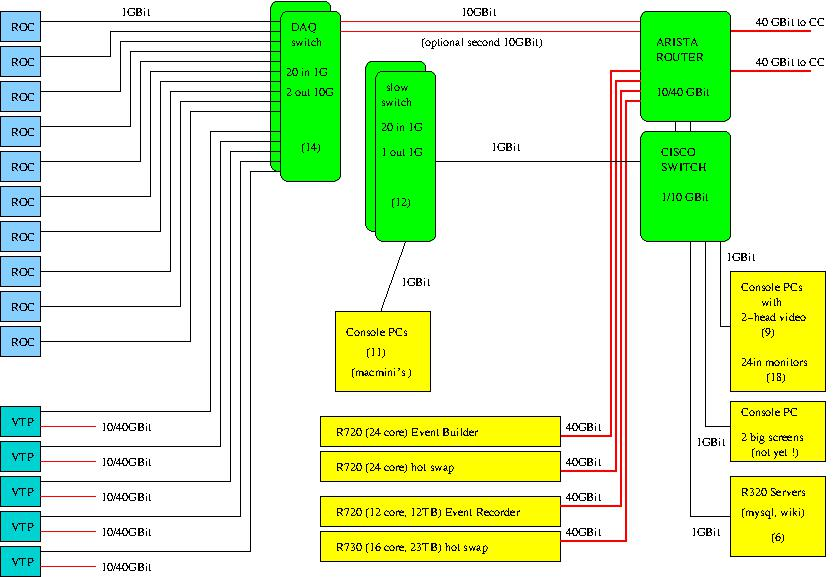
\includegraphics[width=1.0\columnwidth,keepaspectratio]{img/CLAS12_NET_1.jpg}
	\caption{CLAS12 DAQ Network Diagram. All components and connections have adequate performance for the
          currently running and planned experiments.}
	\label{fig:network_diagram}
\end{figure}
